\chapter{A Unified Model for Multi-Modal Attention} 
\label{chapter-unified} 

In Section \ref{sec:background-attention}, three types of multi-modal attention in humans were discussed i.e., endogenous, exogenous and crossmodal attention \citep{crossmodal}. As a reminder, attention is endogenous when we \textit{voluntary} choose to attend to something whereas exogenous orients occurs when a person's attention is captured \textit{reflexively} by the sudden onset of an unexpected event \citep{crossmodal}. Many exogenous and crossmodal attention mechanisms have been developed in MMDL in recent years \citep{attention-need, cross-transformer}. By contrast, at the best of our knowledge no previous study has investigated exogenous attention mechanism in deep learning. The EMMA module was created to close this gap. Indeed, EMMA handles unexpected situations by focusing instead on the most relevant modes.

\begin{figure}[hbt!]
\centering
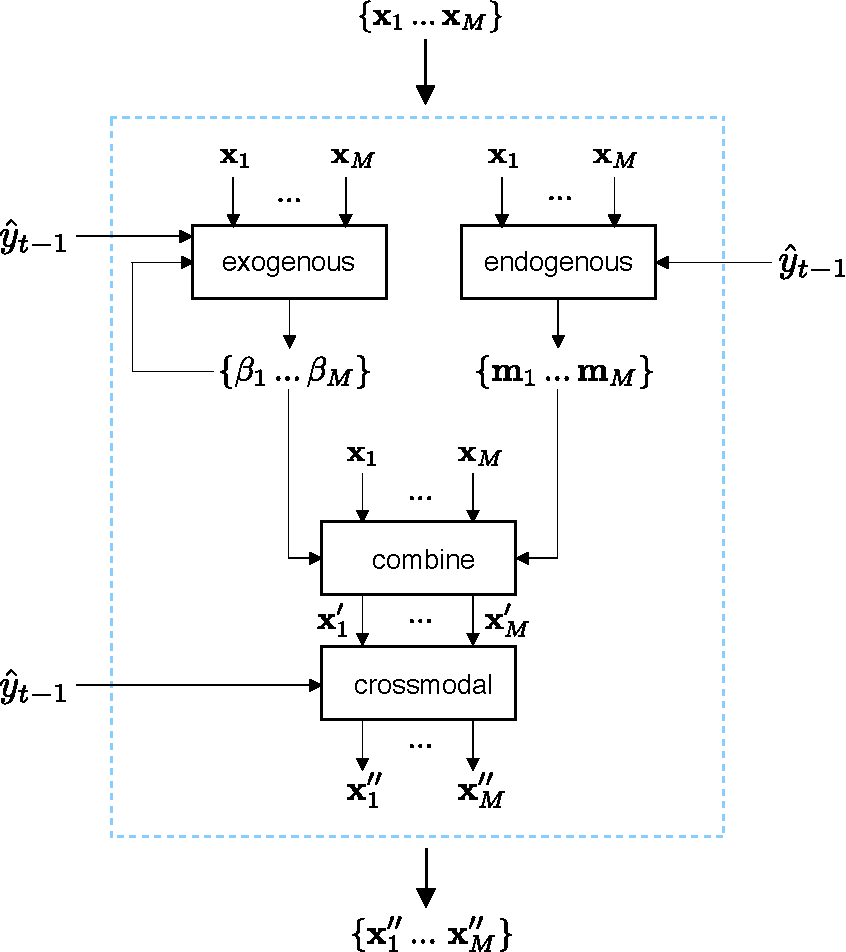
\includegraphics[scale=0.6]{figures/unified}
\vspace*{1cm}
\caption{A general model for Multi-Modal Attention}
\label{fig:complete-model}
\end{figure}

Three attention mechanisms at our disposal could be used to construct a complete Multi-Modal attention (see Figure \ref{fig:complete-model}). First, the multi-modal input is forwarded in parallel through an exo- and endogenous module. The exogenous module outputs attention scores as in Chapter \ref{chapter-emma}. In a similar way, the endogenous module outputs attention masks, where each mask is structured as the corresponding mode and indicates where to focus attention inside the mode. The scores and masks are multiplied and applied to the input. To refine the result is processed by the crossmodal component, leveraging the intrinsic links between the modes to focus on the most important information. In many real-world scenarios, inputs appear in the form of sequences (e.g. time, text, ...). Under those circumstances, the unified model can be further refined by sending the predicting made for the previous input to the attention modules.

In summary, the exogenous module masks perturbations, the endogenous module learns to attend to important information inside each mode, and the crossmodal extracts knowledge by looking at the whole picture.

%\newpage
%\null
%\vfill
%\begin{center}
%\begin{figure}[hbt!]
%\centering
%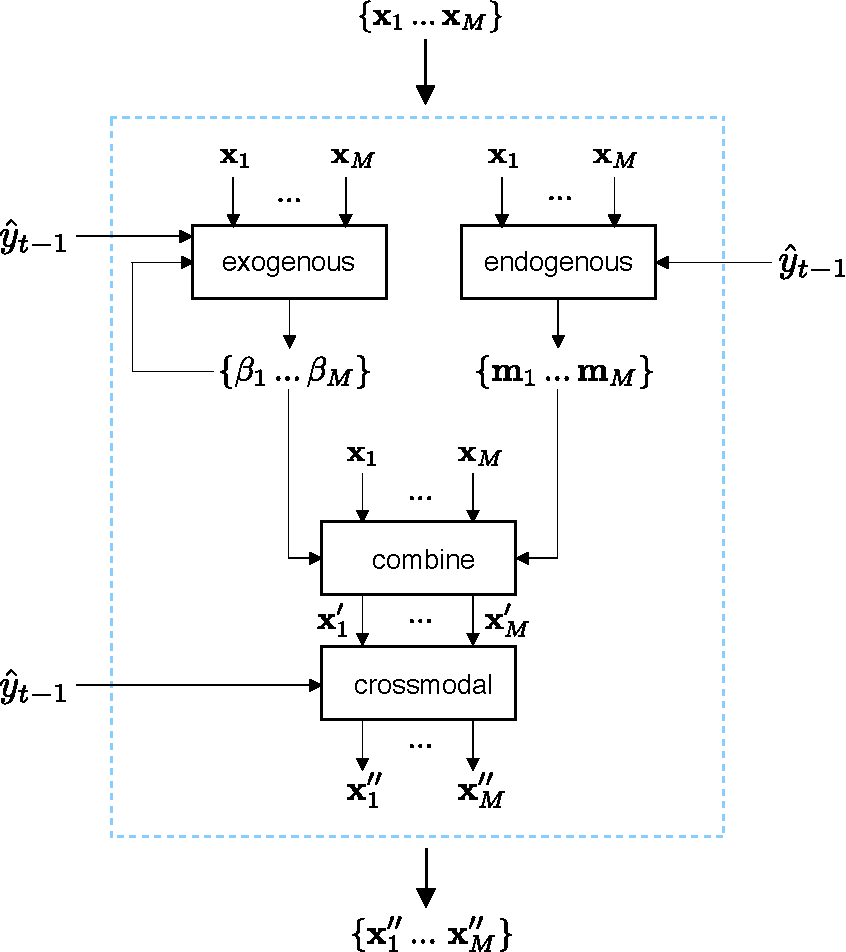
\includegraphics[scale=0.85]{figures/unified}
%\vspace*{1cm}
%\caption{A general model for Multi-Modal Attention}
%\label{fig:complete-model}
%\end{figure}
%\end{center}
%\vfill
%\clearpage


